% !TEX TS-program = pdflatex
% !TEX encoding = UTF-8 Unicode

\documentclass[a4paper]{article}

\usepackage[swedish]{babel}
\usepackage[T1]{fontenc}
\usepackage[utf8]{inputenc}
\usepackage[pdftex]{graphicx}
\usepackage{float}
\usepackage{fancyhdr}
\usepackage[toc,page]{appendix}
\usepackage{booktabs} % for much better looking tables
\usepackage{array} % for better arrays (eg matrices) in maths
\usepackage{paralist} % very flexible & customisable lists (eg. enumerate/itemize, etc.)
\usepackage{verbatim} % adds environment for commenting out blocks of text & for better verbatim
\usepackage{subfig} % make it possible to include more than one captioned figure/table in a single float


%%% HEADERS & FOOTERS
\author{Jonathan Karlsson, Niclas Olofsson, Paul Nedstrand\\jonka293, nicol, paune\\Grupp 2}
\pagestyle{fancy} % options: empty , plain , fancy
\renewcommand{\headrulewidth}{1pt} % customise the layout...
\fancyhead[LO,LE]{Jonathan, Niclas, Paul\\Rapport lab 2-3}
\lfoot{}\cfoot{\thepage}\rfoot{}

%%%% SECTION TITLE APPEARANCE
%\usepackage{sectsty}
%\allsectionsfont{\sffamily\mdseries\upshape} % (See the fntguide.pdf for font help)
%% (This matches ConTeXt defaults)
%
%%%% ToC (table of contents) APPEARANCE
%\usepackage[nottoc,notlof,notlot]{tocbibind} % Put the bibliography in the ToC
%\usepackage[titles,subfigure]{tocloft} % Alter the style of the Table of Contents
%\renewcommand{\cftsecfont}{\rmfamily\mdseries\upshape}
%\renewcommand{\cftsecpagefont}{\rmfamily\mdseries\upshape} % No bold!

%%% END Article customizations

%%% The "real" document content comes below...

\title{Rapport lab 2-3\\ \vspace{2 mm} {\large TSEA44}}
%\date{} % Activate to display a given date or no date (if empty),
         % otherwise the current date is printed 

\begin{document}
\maketitle

\newpage

\tableofcontents

\newpage
\section{Labb 2}
\subsection{Introduktion}
Introduction
\subsection{Tillståndsgraf och arkitektur}
Design, where you explain with text and diagrams how your design works
\subsection{Resultat}
Results, that you have measured
\subsection{Sammanfattning}
Conclusions

Vi följde labbanvisningen och hade ett blockminne med indatan där vi i labb 2 tog data och adress till inminnet direkt från wishbone bussen. Vi tar emot data så fort vi blir adresserade och inväntar en startsignal, när den kommer startar vi en räknare och sätter igång diverse statusflaggor. Räknaren är för att hålla koll på hur många pixlar vi har läst in till DCT \rq{}n. Figur \ref{fig:architecture} visar vad som händer 

\begin{figure}[h]
\centering
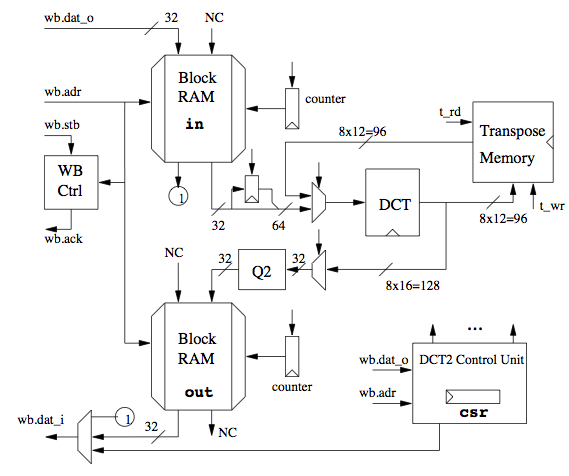
\includegraphics[scale=0.5]{architecture.png}
\caption{Arkitektur för vår design}
\label{fig:architecture}
\end{figure}

hej
\begin{figure}[h]
\centering
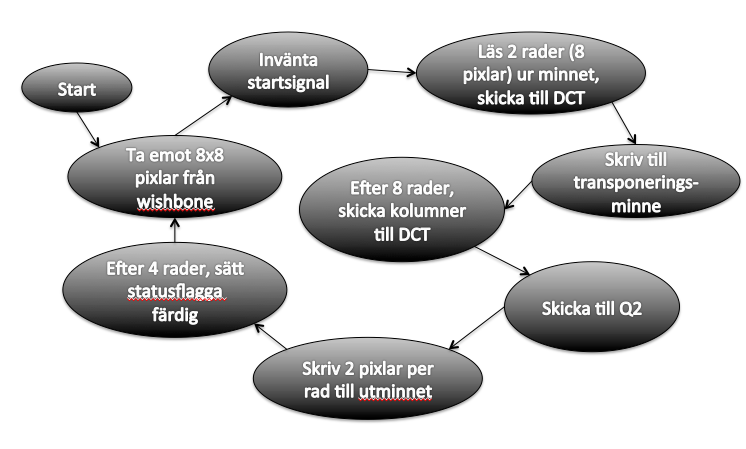
\includegraphics[width=340px]{states.png}
\caption{Tillståndsgraf för vår design}
\label{fig:state}
\end{figure}


\subsection{Filer}

\section{Labb 3}
\subsection{Introduktion}
Introduction
\subsection{Design}
Design, where you explain with text and diagrams how your design works
\subsection{Resultat}
Results, that you have measured
\subsection{Sammanfattning}

\section{What to Include in the Lab Report 2}
The lab report should contain all source code that you have written. (The source code should of course be commented.) We would also like you to include a block diagram of your hardware. If you have written any FSM you should include a state diagram graph of the FSM.
We would also like you to discuss the following questions in detail somewhere in your lab report.
\begin{itemize}
\item How does your 2D DCT hardware work?
\item How did you verify that your 2D DCT hardware works correctly?
\item What is the performance with and without the 2D DCT hardware? This should include measurements of both the 2D DCT kernel and the entire application.
\item A timestamp diagram.
\item How much of the FPGA is used by the 2D DCT hardware?
\item How much is the 2D DCT hardware used while encoding an image in jpegtest?
\item Isthesizeofthe2DDCThardwarejustifiedbytheperformanceimprovements?
\item What would be required in order to implement more functionality like zigzag addressing in the 2D DCT hardware module? Would it be difficult to modify jpegfiles to take advantage of such optimizations?
And of course, the normal parts of a lab report such as a table of contents, an intro- duction, a conclusion, etc. The source code that you have written should be included in appendices and referred to from the main document.
\end{itemize}


\section{What to Include in the Lab Report 3}
The lab report should contain all source code that you have written. (The source code should of course be commented.) We would also like you to include a block diagram of your hardware. If you have written any FSM you should include a state diagram graph of the FSM.
We would also like you to discuss the following questions in detail somewhere in your lab report1:
\begin{itemize}
\item How does your hardware work?
\item How did you verify that your hardware worked?
\item How did you modify the software?
\item A timing diagram.
\item What is the utilization of your accelerator?
\item What is the performance of jpegtest with DMA enabled?
\item How long does it take (on average) to read a macroblock into the DCT acceler- ator via DMA?
\item How much is the wishbone bus used by the DMA unit and how much is the bus used by the CPU?
And of course, the normal parts of a lab report such as a table of contents, an intro- duction, a conclusion, etc. The source code that you have written should be included in appendices and referred to from the main document.
\end{itemize}


\begin{table}[h]
	\centering
 	\begin{tabular}{l l l l}
		stakeholders 			& change1 	& change2  	& change3 \\
		stakeholder1 			& + / -		& + / -		& + / - \\
		stakeholder2 			& + / -		& + / -		& + / - \\
		stakeholder3 			& + / -		& + / -		& + / - \\
	\end{tabular}
	
	\caption{Shows how the different stakeholders are affected by each change.}
	\label{tab:table1}
\end{table}

\begin{table}[h]
	\centering
 	\begin{tabular}{l l l}
	    change1 & description & description \\
	    change2 & description & description \\
	    change3 & description & description \\
	\end{tabular}
	
	\caption{Describes the changes and why they effect the stakeholders.}
	\label{tab:table1}
\end{table}

\begin{appendices}
\section{kod.sv}
\section{kod.sv}
\section{kod.sv}
\end{appendices}

\end{document}
